%%% License: Creative Commons Attribution Share Alike 4.0 (see https://creativecommons.org/licenses/by-sa/4.0/)
%%% Slides are based heavily on earlier versions of this course taught by Jesper Rudiger.

\documentclass[english,10pt
%,handout
,aspectratio=169
]{beamer}
%%% License: Creative Commons Attribution Share Alike 4.0 (see https://creativecommons.org/licenses/by-sa/4.0/)
%%% Slides are based heavily on earlier versions of this course taught by Jesper Rudiger and Peter Norman Sorensen.

\DeclareGraphicsExtensions{.eps, .pdf,.png,.jpg,.mps,}
\usetheme{reMedian}
\usepackage{parskip}
\makeatother

\renewcommand{\baselinestretch}{1.1} 

\usepackage{amsmath, amssymb, amsfonts, amsthm}
\usepackage{enumerate}
\usepackage{hyperref}
\usepackage{url}
\usepackage{bbm}
\usepackage{color}

\usepackage{tikz}
\usepackage{tikzscale}
\newcommand*\circled[1]{\tikz[baseline=(char.base)]{
		\node[shape=circle,draw, inner sep=-20pt] (char) {#1};}}
\usetikzlibrary{automata,positioning}
\usetikzlibrary{decorations.pathreplacing}
\usepackage{pgfplots}
\usepgfplotslibrary{fillbetween}
\usepackage{graphicx}

\usepackage{setspace}
%\thinmuskip=1mu
%\medmuskip=1mu 
%\thickmuskip=1mu 


\usecolortheme{default}
\usepackage{verbatim}
\usepackage[normalem]{ulem}

\usepackage{apptools}
\AtAppendix{
	\setbeamertemplate{frame numbering}[none]
}
\usepackage{natbib}




\title{Financial Markets Microstructure \\ Exercises after L2}

\author{Egor Starkov}

\date{K{\o}benhavns Unversitet \\
	Spring 2022}



\begin{document}
	\AtBeginSection[]{
	\frame<beamer>{
		\frametitle{This lecture:}
		\tableofcontents[currentsection,currentsubsection]
	}}

\frame[plain]{\titlepage}



\section{Problems from Lecture 2}

\begin{frame}{Lecture 2}
From Lecture 2: 
\begin{itemize}
	\item problems 1 and 8 from FRP ch.2 (pp.72-76)
	\item reproduce graphs from lecture ($\approx$ problems 6-7 from FPR ch.2) -- we did that in lecture (duh)
\end{itemize}
\end{frame}


\begin{frame}{Problem 1: Market Depth}
\begin{figure}
	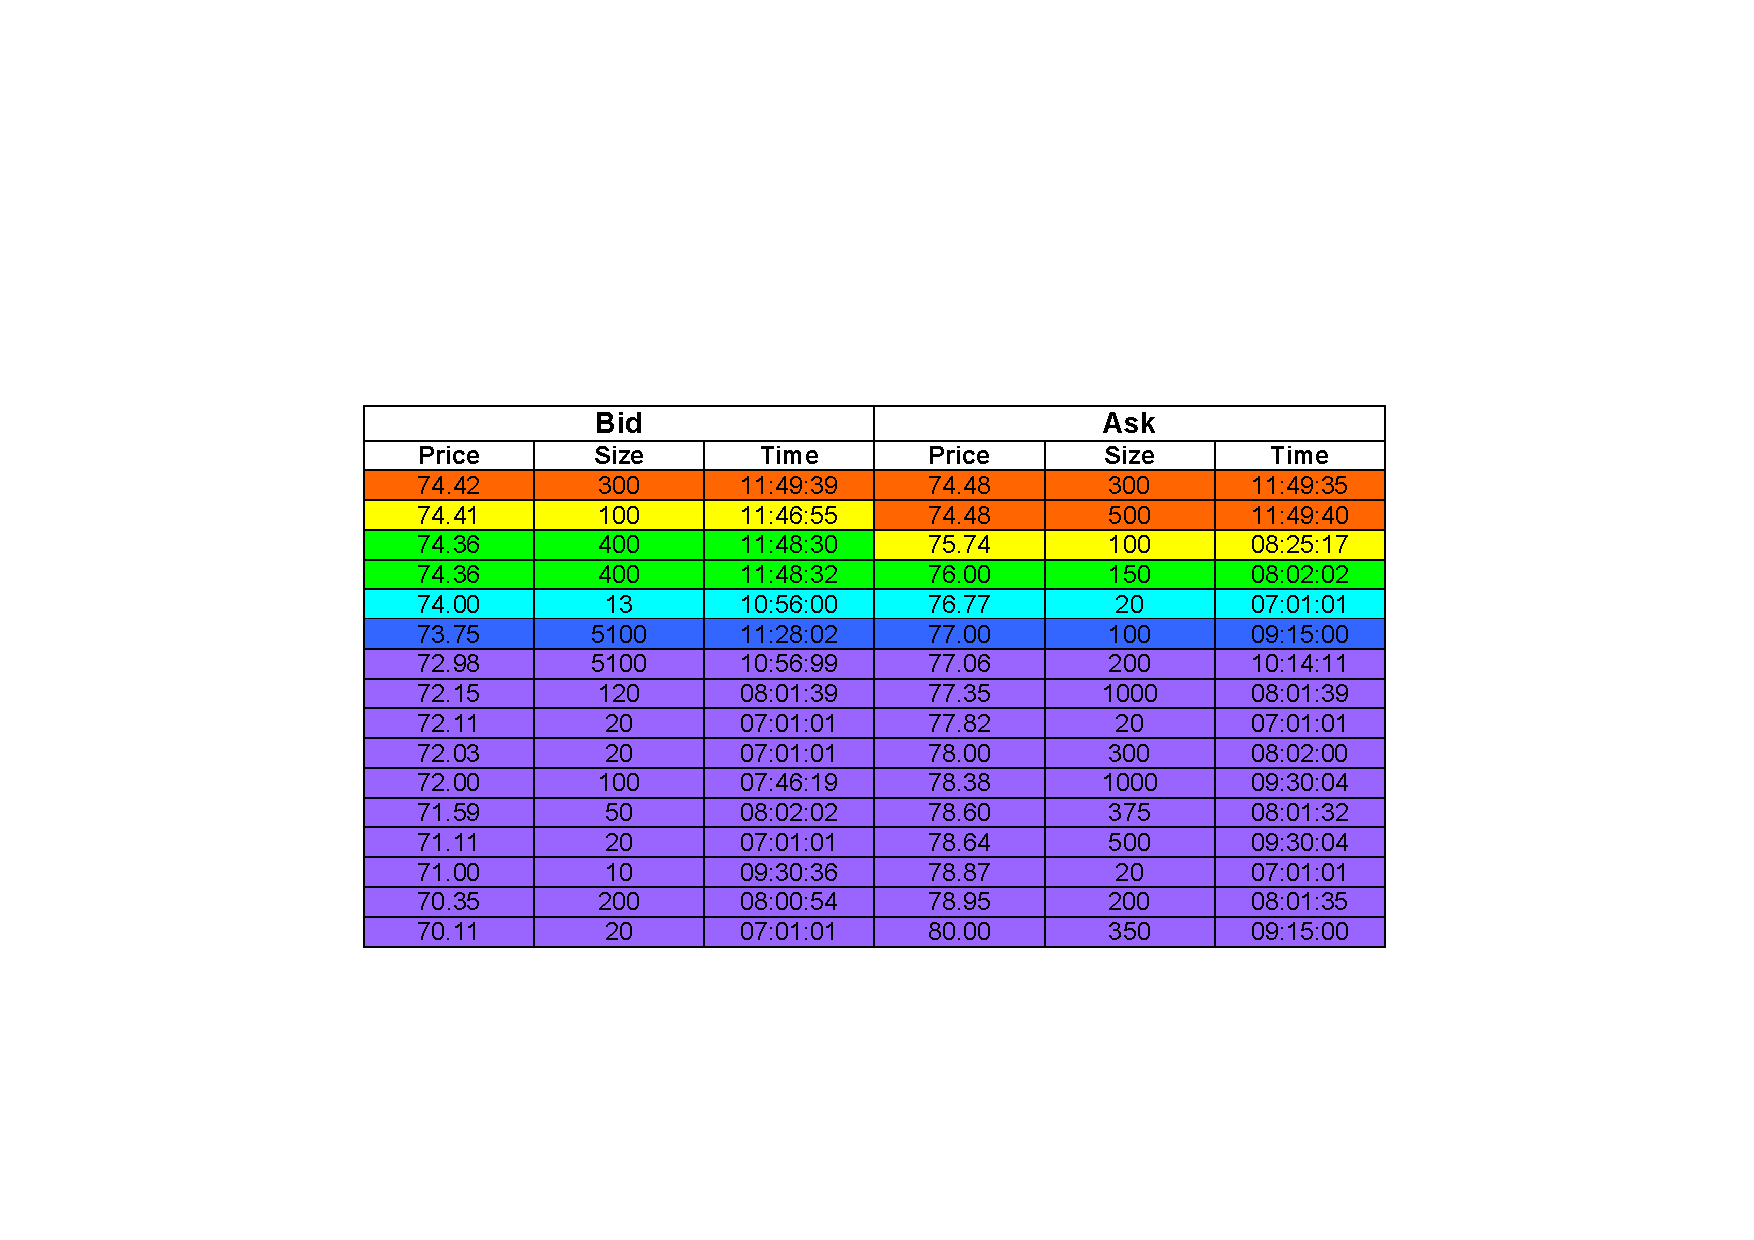
\includegraphics[width=.7\paperwidth]{pics/Image_LOB}
\end{figure}
\end{frame}


\begin{frame}{Problem 1: Market Depth}
	Quoted spreads for different volumes:
	\begin{figure}
		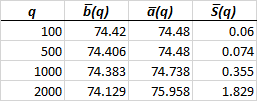
\includegraphics[width=.5\paperwidth]{pics/ch2ex1}
	\end{figure}
	
\end{frame}


\begin{frame}{Problem 1: Market Depth}
\begin{figure}
	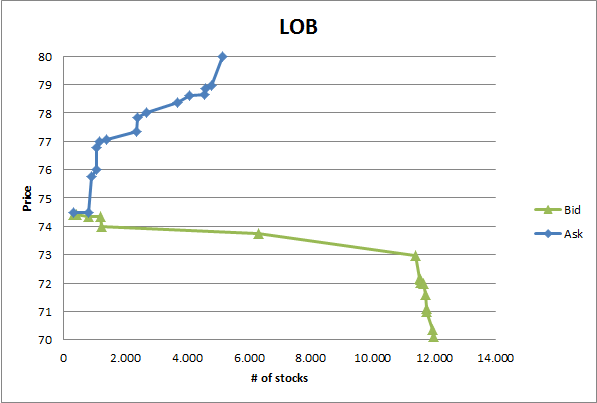
\includegraphics[width=.7\paperwidth]{pics/Graph_LOB}
\end{figure}
\end{frame}


\begin{frame}{Problem 8: Implementation Shortfall}
	\begin{quotation}
		Your client wants to buy $q$ shares in company XYZ at time $0$ and hold them until time $t$. Midprice at time $0$ is $m_0$. Market is not perfectly liquid, so realized [average] purchase price will be $\bar{p} = m_0 + \lambda k q$, where $k \in [0,1]$ is the share of the order fulfilled, $\lambda$ price pressure parameter. Expected midprice at time $t$ is $m_t$ (independent of $k$).
		
		Choose $k$ to minimize the resulting implementation shortfall.
	\end{quotation}
\end{frame}


\begin{frame}{Problem 8: Implementation Shortfall}
	Implementation shortfall:
	\begin{align*}
		IS_t 
		& = q(m_t-m_0) - k q (m_t - \bar{p}) 
		\\
		& = k q(\bar{p} - m_0) + (1-k) q (m_t - m_0)
		\\
		& = \lambda (k q)^2 + (1-k) q (m_t - m_0).
	\end{align*}
	\pause
	Find min:
	\begin{align*}
		\frac{d IS_t(k)}{dk} &= 2 \lambda q^2 k - q (m_t - m_0) = 0
		\\
		\Leftrightarrow k &= \frac{m_t - m_0}{2\lambda q}
	\end{align*}
	(don't forget to check the second order condition: $\frac{d^2 IS_t(k)}{dk^2} > 0$)
\end{frame}


\begin{frame}{Problem 8: Implementation Shortfall}
	$$ k = \frac{m_t - m_0}{2\lambda q} $$
	\begin{itemize}
		\item Increasing in $m_t - m_0$:
		\begin{itemize}
			\item if asset price is expected to increase, the opportunity cost (regret) of not buying the asset is high.
		\end{itemize}
		\item Decreasing in $\lambda$:
		\begin{itemize}
			\item the more sensitive is the price, the less you can buy cheaply enough
		\end{itemize}
		\item Decreasing in $q$:
		\begin{itemize}
			\item (same as above) large orders move prices by more -- costlier to fulfill fully.
		\end{itemize}
	\end{itemize}
\end{frame}


\begin{frame}{Problem 8: Implementation Shortfall}
	\begin{itemize}
		\item If you were solving this problem in reality, you would not know $m_t$.
		\item Instead, treat $m_t$ as your \structure{expectation} of the future price, choose trading strategy to minimize the \structure{expected implementation shortfall}.
	\end{itemize}
\end{frame}

\end{document} 